%%%%%%%%%%%%%%%%%%%%%%%%%%%%%%%%%%%%%%%%%
% Beamer Presentation
% LaTeX Template
% Version 1.0 (10/11/12)
%
% This template has been downloaded from:
% http://www.LaTeXTemplates.com
%
% License:
% CC BY-NC-SA 3.0 (http://creativecommons.org/licenses/by-nc-sa/3.0/)
%
%%%%%%%%%%%%%%%%%%%%%%%%%%%%%%%%%%%%%%%%%

%----------------------------------------------------------------------------------------
%	PACKAGES AND THEMES
%----------------------------------------------------------------------------------------

\documentclass{beamer}

\mode<presentation> {

% The Beamer class comes with a number of default slide themes
% which change the colors and layouts of slides. Below this is a list
% of all the themes, uncomment each in turn to see what they look like.

%\usetheme{default}
%\usetheme{AnnArbor}
%\usetheme{Antibes}
%\usetheme{Bergen}
%\usetheme{Berkeley}
%\usetheme{Berlin}
%\usetheme{Boadilla}
%\usetheme{CambridgeUS}
%\usetheme{Copenhagen}
%\usetheme{Darmstadt}
%\usetheme{Dresden}
%\usetheme{Frankfurt}
%\usetheme{Goettingen}
%\usetheme{Hannover}
%\usetheme{Ilmenau}
%\usetheme{JuanLesPins}
%\usetheme{Luebeck}
\usetheme{Madrid}
%\usetheme{Malmoe}
%\usetheme{Marburg}
%\usetheme{Montpellier}
%\usetheme{PaloAlto}
%\usetheme{Pittsburgh}
%\usetheme{Rochester}
%\usetheme{Singapore}
%\usetheme{Szeged}
%\usetheme{Warsaw}

% As well as themes, the Beamer class has a number of color themes
% for any slide theme. Uncomment each of these in turn to see how it
% changes the colors of your current slide theme.

%\usecolortheme{albatross}
%\usecolortheme{beaver}
%\usecolortheme{beetle}
%\usecolortheme{crane}
\usecolortheme{dolphin}
%\usecolortheme{dove}
%\usecolortheme{fly}
%\usecolortheme{lily}
%\usecolortheme{orchid}
%\usecolortheme{rose}
%\usecolortheme{seagull}
%\usecolortheme{seahorse}
%\usecolortheme{whale}
%\usecolortheme{wolverine}

%\setbeamertemplate{footline} % To remove the footer line in all slides uncomment this line
%\setbeamertemplate{footline}[page number] % To replace the footer line in all slides with a simple slide count uncomment this line

%\setbeamertemplate{navigation symbols}{} % To remove the navigation symbols from the bottom of all slides uncomment this line
}
\usepackage{array} 
\usepackage{graphicx} % Allows including images
\usepackage{booktabs} % Allows the use of \toprule, \midrule and \bottomrule in tables

%----------------------------------------------------------------------------------------
%	TITLE PAGE
%----------------------------------------------------------------------------------------

\title[Hiter inženiring]{Hiter inženiring pri razvoju programske opreme} % The short title appears at the bottom of every slide, the full title is only on the title page

\author{Svit Spindler} % Your name
\institute[FRI] % Your institution as it will appear on the bottom of every slide, may be shorthand to save space
{
Univerza v Ljubljani \\ % Your institution for the title page
\medskip
\textit{svit.spindler@gmail.com} % Your email address
}
\date{\today} % Date, can be changed to a custom date

\begin{document}

\begin{frame}
\titlepage % Print the title page as the first slide
\end{frame}

\begin{frame}
\frametitle{Overview} % Table of contents slide, comment this block out to remove it
\tableofcontents % Throughout your presentation, if you choose to use \section{} and \subsection{} commands, these will automatically be printed on this slide as an overview of your presentation
\end{frame}

%----------------------------------------------------------------------------------------
%	PRESENTATION SLIDES
%----------------------------------------------------------------------------------------
\section{Uvod}
\begin{frame}
\frametitle{Uvod}
Orodja za dopolnjevanje in generiranje kode so postala zelo priljubljena pri programiranju, saj omogočajo hitrejše in učinkovitejše reševanje problemov. Med najbolj znanimi orodji so GitHub Copilot, Amazon CodeWhisperer in ChatGPT podjetja OpenAI, ki jih uporabljajo tako začetniki kot izkušeni programerji. Namen te študije je preučiti prednosti in slabosti teh orodij ter njihov vpliv na proces učenja in programiranja pri začetnikih, z osredotočanjem na hitrost in kvaliteto kode v jeziku Python.
\end{frame}

%------------------------------------------------
\section{Cilj naloge}
\begin{frame}
\frametitle{Cilj naloge}
\begin{itemize}
\item Raziskati prednosti in slabosti hitrega inženiringa
\item Raziskati različna orodja umetne inteligence
\item Primerjava različnih orodij za hiter inženiring
\item Raziskati vpliv hitrega inženiringa pri začetnih programerjih
\end{itemize}
\end{frame}

%------------------------------------------------

\begin{frame}
\frametitle{Table}
\begin{table}
\centering
\caption{Primerjava orodij ChatGPT, GitHub Copilot in Amazon CodeWhisperer}
\small % Reduce text size
\renewcommand{\arraystretch}{1.2} % Adjust row height
\begin{tabular}{|>{\raggedright\arraybackslash}p{2.8cm}|>{\raggedright\arraybackslash}p{2.2cm}|>{\raggedright\arraybackslash}p{2.2cm}|>{\raggedright\arraybackslash}p{2.5cm}|}
\hline
\textbf{Lastnost} & \textbf{ChatGPT} & \textbf{GitHub Copilot} & \textbf{Amazon CodeWhisperer} \\ \hline
Razvijalec & OpenAI & OpenAI-Microsoft & AWS \\ \hline
Datum izdaje & 30. 11. 2022 & 29. 10. 2021 & 23. 06. 2022 \\ \hline
Razlaga kode & Da & Da & Ne \\ \hline
\end{tabular}
\label{tab:comparison}
\end{table}
\end{frame}

%------------------------------------------------
\section{Metodologija}
\begin{frame}
\frametitle{Metodologija}
Namen diplomskega dela je bil raziskati, kako hiter inženiring vpliva na proces razvoja programske opreme, s preučevanjem hitrosti in kvalitete kode pri uporabi orodij umetne inteligence. Najprimernejša metoda za pridobivanje teh podatkov je bil nadzorovan eksperiment na skupini mlajših otrok, ker omogoča natančen nadzor nad spremenljivkami ter izolirano vrednotenje reševanja programskih problemov.
\end{frame}

%------------------------------------------------
\section{Načrt}
\begin{frame}
\frametitle{Načrt}
\begin{figure}
    \centering
    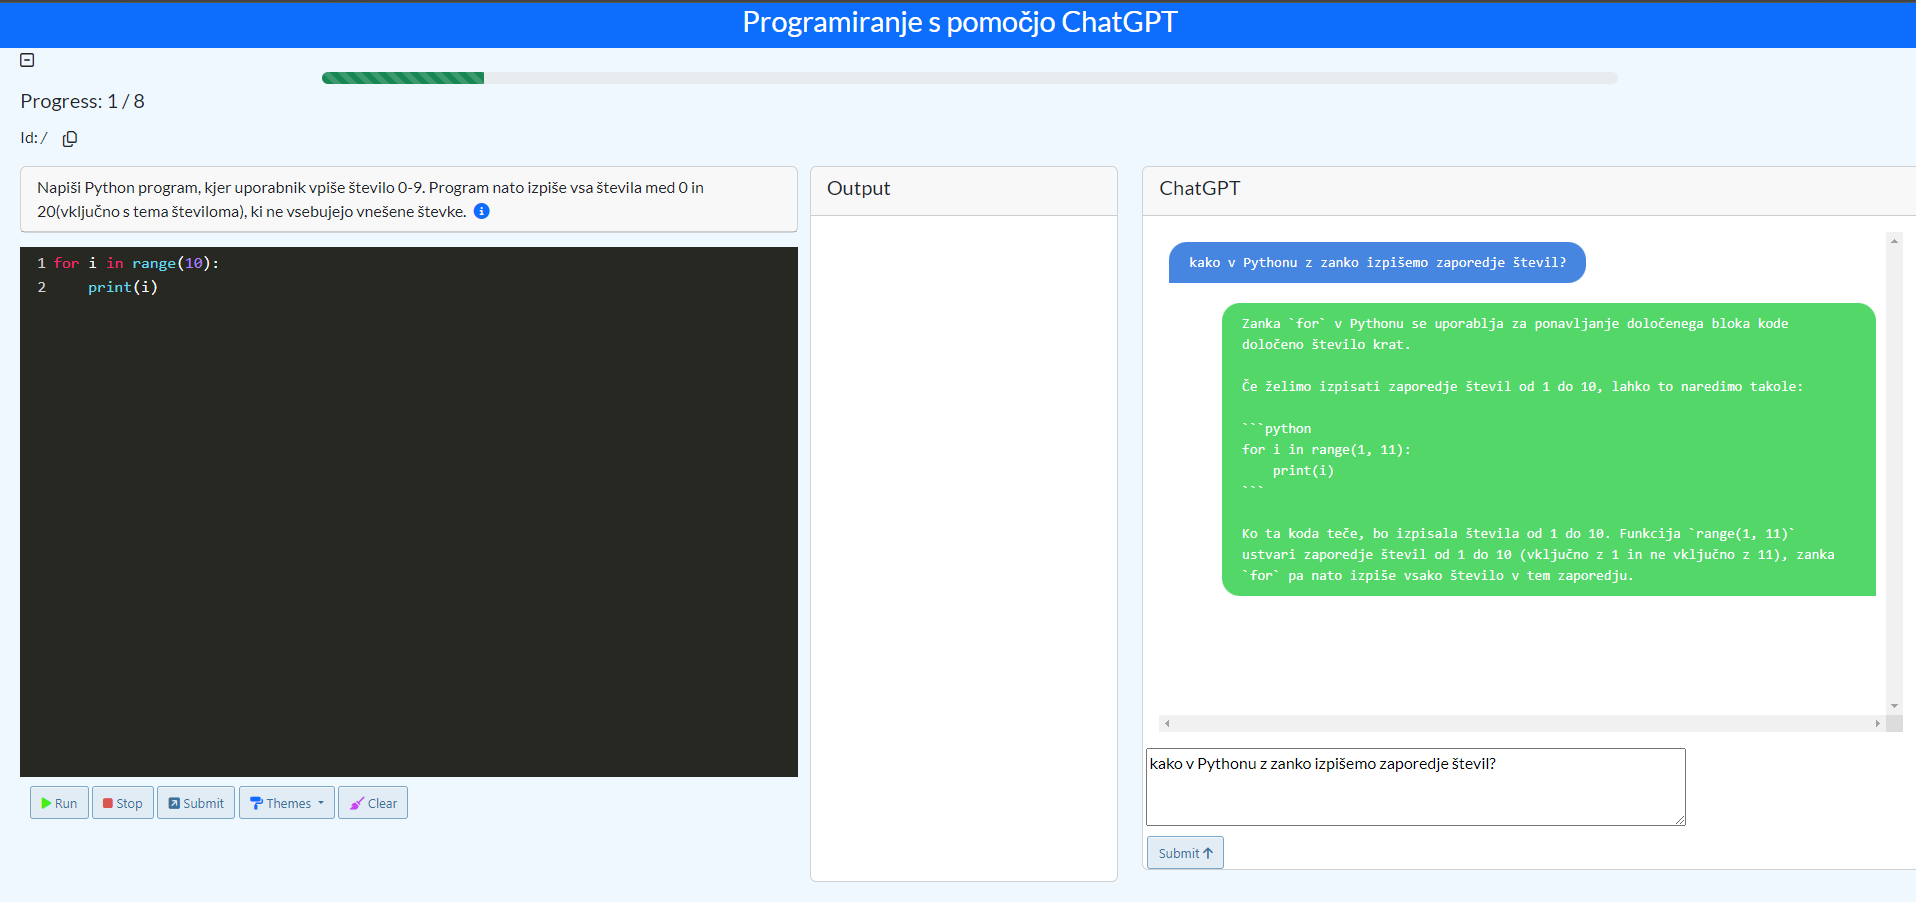
\includegraphics[width=1\linewidth]{spletna_stran.png}
    \caption{Spletna stran eksperimenta}
    \label{fig:enter-label}
\end{figure}
\end{frame}

%------------------------------------------------

\begin{frame}
\frametitle{Načrt}
Za izvedbo eksperimenta smo izbrali več skupin mlajših otrok, ki se učijo programiranja v jeziku Python. Za namen eksperimenta je bila razvita preprosta spletna stran, ki je imela navodila za različne naloge, prostor za pisanje Python kode z označevanjem sintakse, prostor za izpis izhoda programa ter prostor za pogovor z uporabo ChatGPT-3.5
\end{frame}

%------------------------------------------------
\section{Izvedba}
\begin{frame}
\frametitle{Izvedba}
Eksperiment je bil izpeljan v štirih skupinah, ena izmed teh je bila v fizični obliki, ostale skupine pa so bile na daljavo. Skupaj je bilo veljavnih 32 podatkov. Eksperiment je potekal tako, da je bilo najprej predstavljena umetna inteligenca in hiter inženiring, ter najboljše prakse za uporabo ChatGPT za pomoč pri programiranju. Nato je bila rešena krajša anketa o predznanju programiranja ter o poznavanju ChatGPT-ja. Po tem so imeli dobro uro za samo reševanje nalog. Med samim eksperimentom se otrokom ni pomagalo, razen z interpretacijo navodil.
\end{frame}

%------------------------------------------------
\section{Ocena}
\begin{frame}
\frametitle{Ocena}
Znotraj enake težavnosti nalog so bile naloge, pri katerih je bila omogočena uporaba pogovornega okna s ChatGPT rešene mnogo hitreje in z manj napakami. 
\end{frame}

%------------------------------------------------

\begin{frame}
\Huge{\centerline{The End}}
\end{frame}

%----------------------------------------------------------------------------------------

\end{document} 